\chapter{Modellierung (10 Seiten)}
\label{sec:modellierung}
\begin{itemize}
    \item aus den Grundlagen \ref{sec:grundlagen} eine Modellierung des optimalen Trainingsplans 
\end{itemize}

Hierbei ist sowohl der Kontext des Plans in der Entwicklung des Sportlers als auch die Ausrichtung (konkreter Wettkampf / jährlicher Plan / monatlicher Plan / ... ) wichtig
Danach fließt in der Phase der konkreten Trainingsplanung die Anforderung und das individuelle Belastungsprofil des Sportlers ein. Regenerationsphasen müssen berücksichtigt werden. 
In der letzten Phase werden die konkreten Trainingseinheiten festgelegt. Diese beinhalten sowohl Trainingsmethoden, als auch Intensität und Dauer der Belastungen. 
Diese Arbeit behandelt ausschließlich die initiale Erstellung eines Trainingsplans. Es erfolgt keine Trainingskontrolle oder Dokumentation.


\section{Vorgehen}
\label{sec:modellierung:vorgehen}
    \subsection{Top Down an Zyklen}
    \begin{figure}[htb]
    	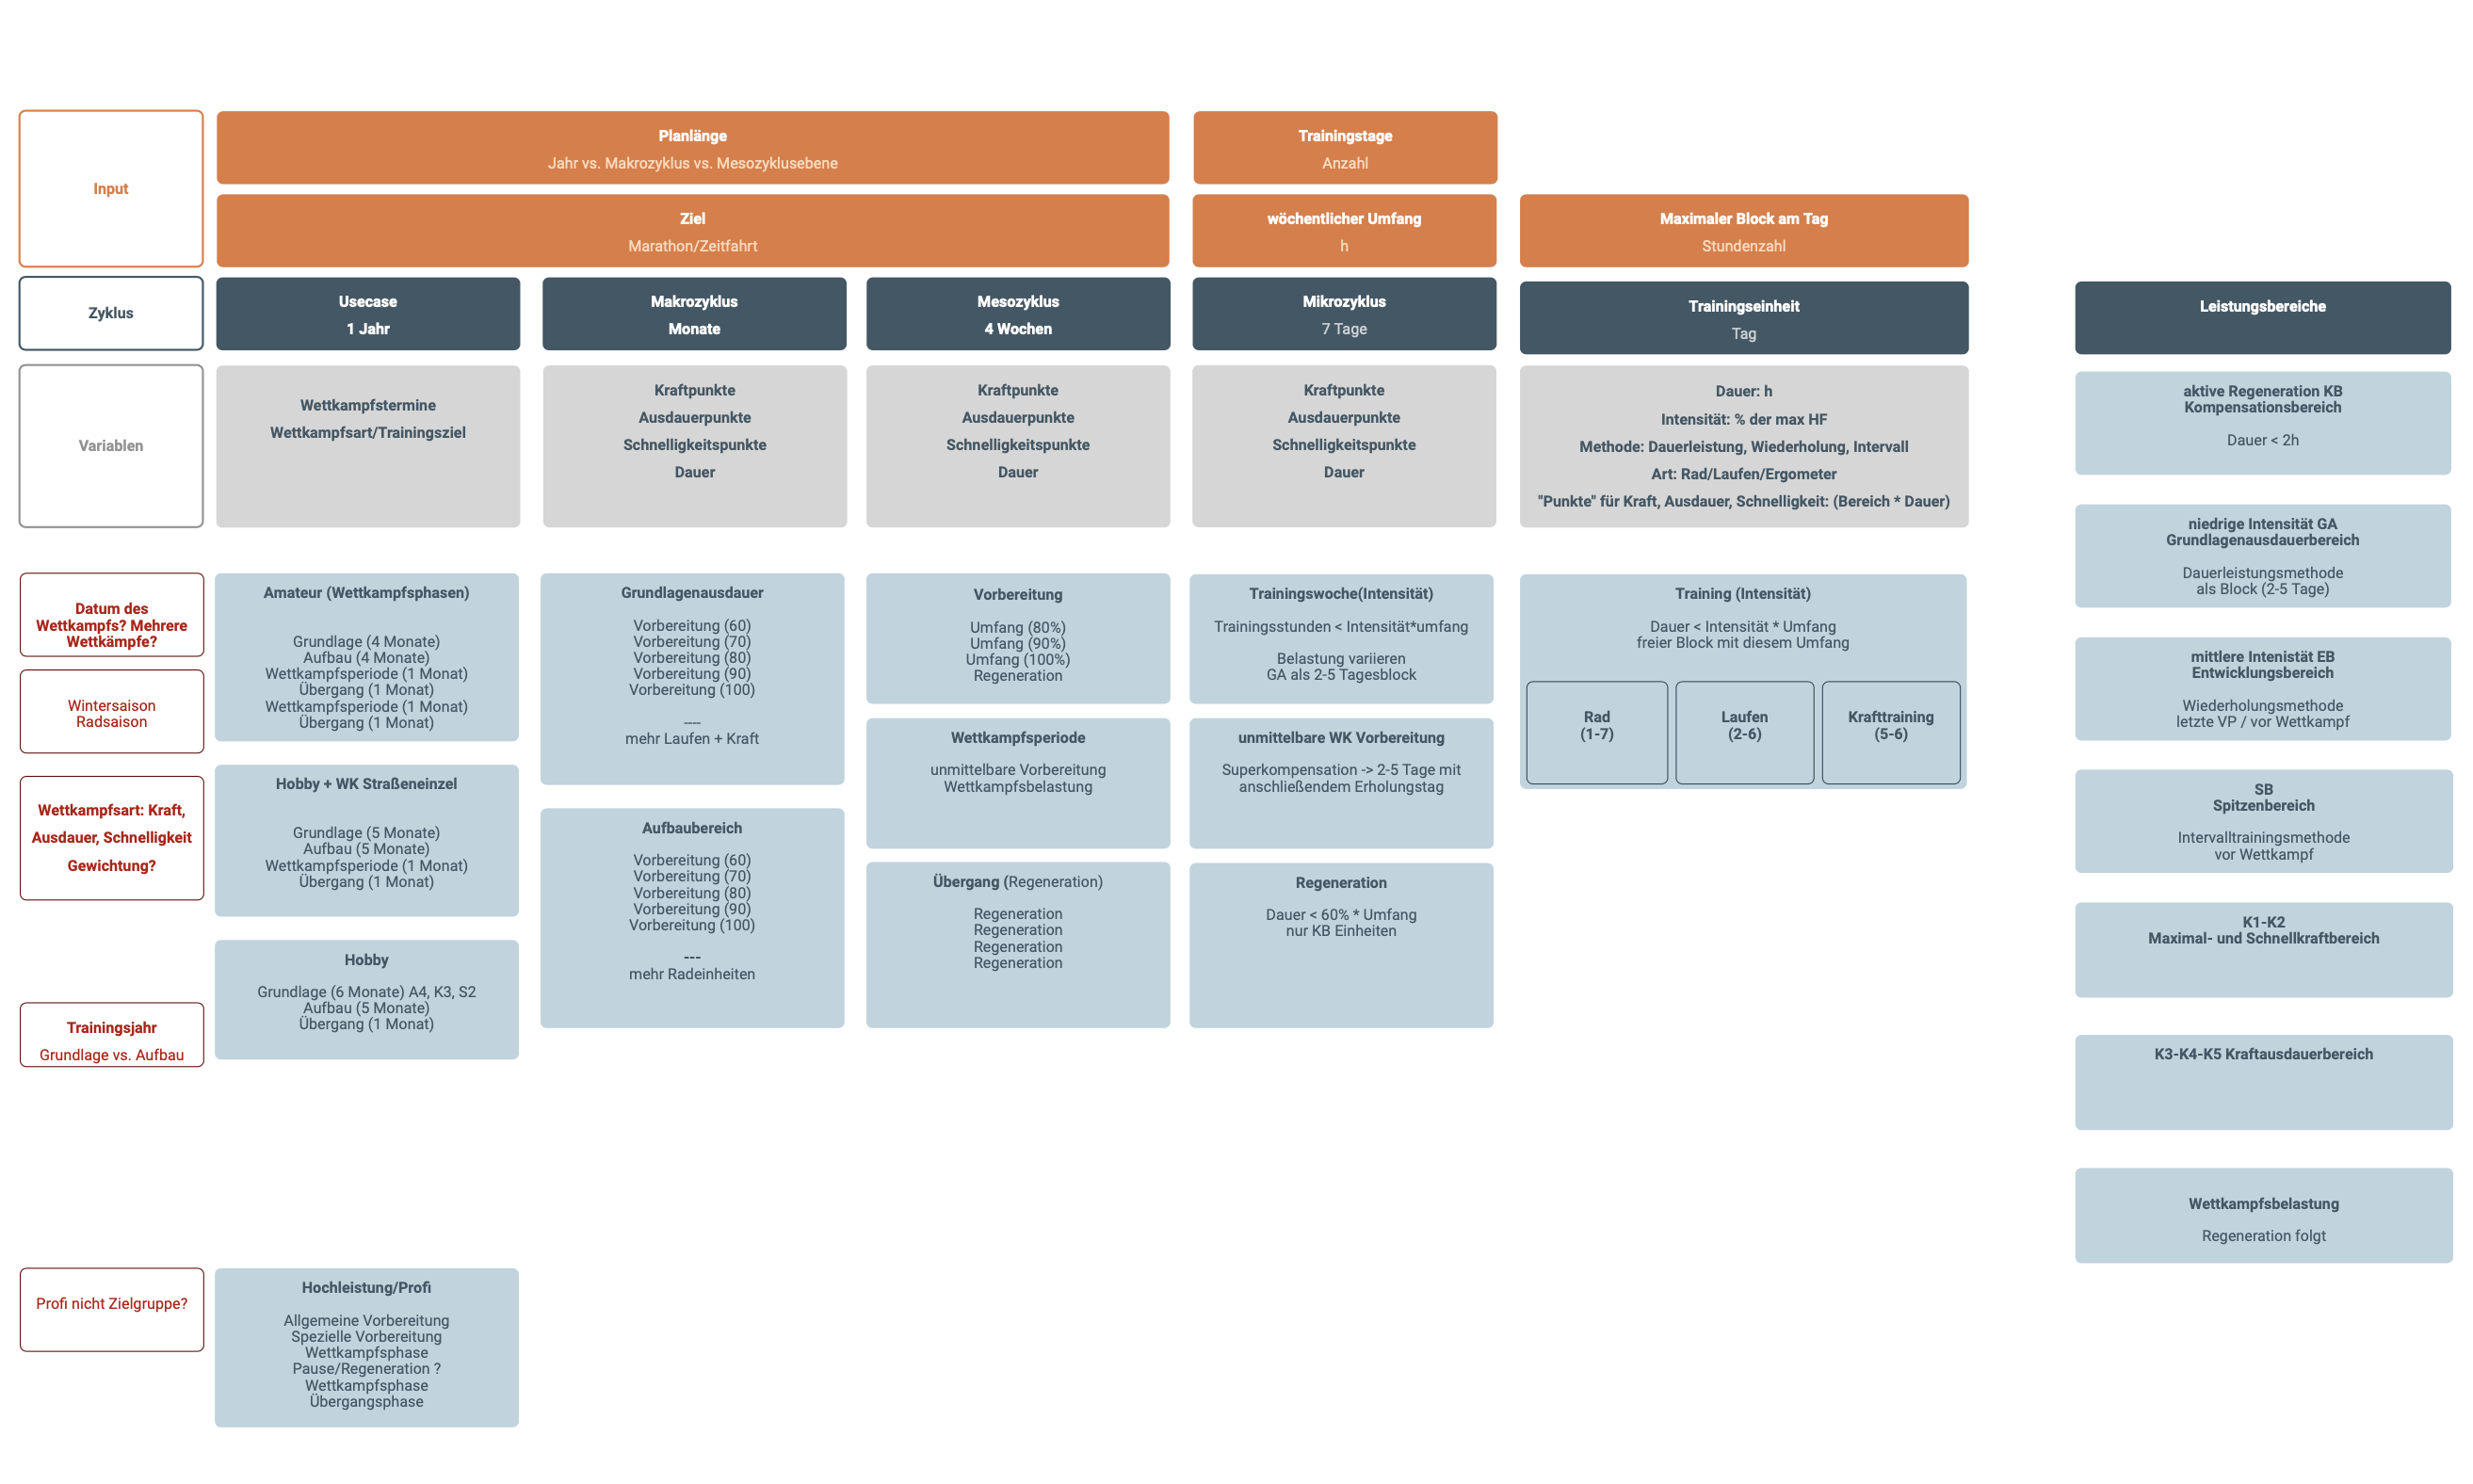
\includegraphics[width=\textwidth]{gfx/modell.png}
    	\caption{Schema der Modellierung}
    	\label{fig:system:example1}
    \end{figure}
    \begin{enumerate}
        \item Zielgruppe bestimmen 
        \item Trainingsziel definieren
        \item Periodisierung durch Wettkämpfe definieren ? Trainingsverlauf (Regeneration auf jeder Stufe einbeziehen einbeziehen)
        \item Constraints auf jeder Ebene der Hierarchie definieren Anteile der einzelnen  Belastungsbereiche an der Trainingsdauer
        \item Trainingseinheiten erstellen
        \item strukturierte Einheit? (z.B. 3km Intervall, Pause)
    \end{enumerate}
    
    
    
\subsection{Scheduling der Trainingseinheiten abhängig vom Kalender}
    \begin{itemize}
        \item Kann man das als getrennten Schritt betrachten? Vorher nur maximale Trainingszeit am Wochentag berücksichtigen
        \item Wie groß ist der Einfluss von Trainingspausen auf die direkte Planung -> st es wichtig zu welcher Zeit an diesem Tag das Training stattfindet? z.B Abends und dann direkt wieder morgens trainieren. 
        \item eventuell schon, wenn z.B. das ganze Wochenende als Regenerationsphase gesetzt sein muss. Reicht es nur Tage zu betrachten, an denen gar nicht trainiert werden kann? 
        \item mindeste Stundenzahl um es als Regenerationsphase zu sehen?
    \end{itemize}
% \subsection{Allgemeines Settings}
% \begin{itemize}
%     \item Trainingsziele: Was soll erreicht werden?
%     \begin{enumerate}
%         \item Wettkampfsvorbereitung
%             \begin{itemize}
%                 \item Vorbereitung mit Gewichtung je nach Streckenprofil
%                 \item Länge
%             \end{itemize}
%         \item Ausdauerfahrt
%         \item Zeitfahrt
%         \item Bergfahrt
%     \end{enumerate}
%     \item Kontext: Wie ist der aktuelle Stand und was folgt?
%     \begin{itemize}
%         \item Vorbereitung -> Jahresplan
%         \item Allgemeine Fitness (Hobbyfahrer ohne Wettkampf)
%         \item Winter/ vs. Sommer/Radsaison -> mehr/weniger Allgemeine Fitness traininieren
%     \end{itemize}
% \end{itemize}

\subsection{Input}
\begin{itemize}
    \item maximaler wöchentlicher Trainingsumfang (h)
    \item Leistungsgruppe \cite[S. 173]{Radsporttraining} (unregelmäßig Trainierende, Ausgleichssportler, Hobbyfahrer ohne Wettkampf, Fahrer mit Wettkämpfen) -> Unterscheiden sich hauptsächlich in "maximaler wöchentlicher Umfang"
    \item Trainingsjahr statt Alter -> \cite[181]{EinfuerungTrainingswissenschaft}
    \item Geschlecht: Welche Auswirkungen hat das?
    \item Gesamtdauer des Plans
        \begin{itemize}
            \item Jahresplan
            \item einzelner Makrozyklus
        \end{itemize}

    \item Disziplin \cite[S.11]{Radsporttraining} (Straßeneinzelrennen, Etappenrennen, Streckenfahrt, Berg/Steigung) mit unterschiedlicher Gewichtung der Trainingsziele \cite[S.14]{Radsporttraining}
\end{itemize}
\subsection{Variablen}

\subsection{Constraints}
    \begin{itemize}
        \item Anzahl der Periodisierung nach Wettkampfsphasen
        \item Gestaltung einer konkreten Trainingseinheit
        \begin{itemize}
            \item es gibt einen freien Zeitslot an diesem Tag
            \item die Verteilung der Trainingsdauer in diesen Bereichen ist eingehalten. Welche Fehlerschranke erlauben?
        \end{itemize}
        \item Trainingsplan
        \begin{itemize}
            \item Nur ein Training am Tag
            \item Nicht mehr als x aufeinanderfolgende Trainingstage
            \item maximal 6 Training in der Woche -> Quelle
            \item GA Trainings am Besten als Block \cite[34]{Radsporttraining}
        \end{itemize}
    \end{itemize}

\subsection{Output - Trainingseinheit}
\label{sec:modellierung:output}
    \begin{itemize}
        \item Tag
        \item Zeitspanne
        \item Dauer/Umfang bzw. Strecke/Zeit 
        \item Trainingsbereich \ref{tab:trainingsbereiche}
        \item zugehöriger Mikro, Meso, Makrozyklus?
        \item Trainingsmethode (eventuell nur Vorschläge: Rad, Laufen, Kraft, aktive Regeneration, ...)
    \end{itemize}